\icode{E-MI-SI-L3-261106-001}
质量为 \( m_1 \) 的楔形斜面体放在水平桌面上，质量为 \( m_2 \) 的小物块以速度 \( v_0 \) 沿斜面匀速下滑。现在物块上分别施加 \( F_1 \) 和 \( F_2 \) 作用，其中 \( F_1 \) 沿水平方向，\( F_2 \) 与斜面夹角为 \( \alpha \)，如图所示，斜面倾角为 \( \theta =\) \,\qty{37}{\degree}，已知\(\sin\)\,\qty{37}{\degree}\(=0.6\)，\(\cos\)\,\qty{37}{\degree}\(=0.8\)，斜面体始终处于静止状态。下列说法正确的是\paren[]
	
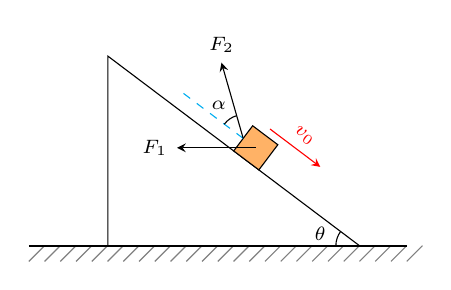
\begin{tikzpicture}[>=stealth,font=\scriptsize]
	\begin{scope}[rotate=-37]
		\draw (0,0)--(-4,0)--++(-53:2.4);
		\draw[fill=orange!60] (-1.6,0) rectangle(-2,.4);
		\coordinate (o) at(-1.8,.2);
		\draw[dashed,cyan] (-2,.2)--++(-1,0);
		\draw[->] (-2,.2)--++(143:1)node[above]{\(F_2\)};
		\draw (-2.3,.2) arc(180:143:.3);
		\draw[->,red] (-1.8,.5)--node[above,rotate=-37]{\(v_0\)}(-1,.5);
		\node at(-2.5,.35){\(\alpha\)};
	\end{scope}
	\draw[->] (o)--++(-1,0)node[left]{\(F_1\)};
	\draw (-.3,0) arc(180:143:.3);
	\foreach \x in {-4.2,-4,...,0.6}
		\draw[gray] (\x,-.2)--++(.2,.2);
	\draw[thick] (-4.2,0)--(.6,0);
	\node at(-.5,.15){\(\theta\)};
\end{tikzpicture}
\begin{choices}
	\item 若仅施加 \( F_1 \) 作用后小物块继续下滑，则此时桌面给斜面体的静摩擦力向左
	\item 若仅施加 \( F_1 \) 作用后小物块继续下滑，则此时桌面给斜面体的静摩擦力向右
	\item 若仅在 \( F_2 \) 作用下小物块沿斜面向上匀速运动，则 \( \alpha \) 等于\qty{37}{\degree}时，\( F_2 \) 最小
	\item 若仅在 \( F_2 \) 作用下小物块沿斜面向上匀速运动，则地面给斜面体的静摩擦力向左
\end{choices}
\begin{answer}
    C\qquad 提示：
\end{answer}